%===============================================================================
% LaTeX sjabloon voor de bachelorproef toegepaste informatica aan HOGENT
% Meer info op https://github.com/HoGentTIN/latex-hogent-report
%===============================================================================

\documentclass[dutch,dit,thesis]{hogentreport}

% TODO:
% - If necessary, replace the option `dit`' with your own department!
%   Valid entries are dbo, dbt, dgz, dit, dlo, dog, dsa, soa
% - If you write your thesis in English (remark: only possible after getting
%   explicit approval!), remove the option "dutch," or replace with "english".

\usepackage{lipsum} % For blind text, can be removed after adding actual content

%% Pictures to include in the text can be put in the graphics/ folder
\graphicspath{{graphics/}}

%% For source code highlighting, requires pygments to be installed
%% Compile with the -shell-escape flag!
\usepackage[section]{minted}
\usepackage{biblatex}
\usepackage{hyperref}
\usepackage{graphicx}
\usepackage{url}
\usepackage{booktabs}
\usepackage{multirow}
\usepackage{listings}

\lstset{language=JavaScript}

%% If you compile with the make_thesis.{bat,sh} script, use the following
%% import instead:
%% \usepackage[section,outputdir=../output]{minted}
\usemintedstyle{solarized-light}
\definecolor{bg}{RGB}{253,246,227} %% Set the background color of the codeframe

%% Change this line to edit the line numbering style:
\renewcommand{\theFancyVerbLine}{\ttfamily\scriptsize\arabic{FancyVerbLine}}

%% Macro definition to load external java source files with \javacode{filename}:
\newmintedfile[javacode]{java}{
    bgcolor=bg,
    fontfamily=tt,
    linenos=true,
    numberblanklines=true,
    numbersep=5pt,
    gobble=0,
    framesep=2mm,
    funcnamehighlighting=true,
    tabsize=4,
    obeytabs=false,
    breaklines=true,
    mathescape=false
    samepage=false,
    showspaces=false,
    showtabs =false,
    texcl=false,
}

% Other packages not already included can be imported here

%%---------- Document metadata -------------------------------------------------
% TODO: Replace this with your own information
\author{Robin De Waegeneer}
\supervisor{Dhr. S. Labijn}
\cosupervisor{Dhr. T. Aelbrecht}
\title[]%
    {Vergelijkende studie van Augmented Reality ondersteunde mobiliteitstool voor personen met een mentale beperking: een proof of concept.}
\academicyear{\advance\year by -1 \the\year--\advance\year by 1 \the\year}
\examperiod{2}
\degreesought{\IfLanguageName{dutch}{Professionele bachelor in de toegepaste informatica}{Bachelor of applied computer science}}
\partialthesis{false} %% To display 'in partial fulfilment'
%\institution{Internshipcompany BVBA.}

%% Add global exceptions to the hyphenation here
\hyphenation{back-slash}
\hyphenation{voor-op}
\hyphenation{tech-no-lo-gieën}
\hyphenation{ef-fi-ciën-tie}

%% The bibliography (style and settings are  found in hogentthesis.cls)
\addbibresource{bachproef.bib}            %% Bibliography file
\addbibresource{../voorstel/voorstel.bib} %% Bibliography research proposal
\defbibheading{bibempty}{}

%% Prevent empty pages for right-handed chapter starts in twoside mode
\renewcommand{\cleardoublepage}{\clearpage}

\renewcommand{\arraystretch}{1.2}

%% Content starts here.
\begin{document}

%---------- Front matter -------------------------------------------------------

\frontmatter

\hypersetup{pageanchor=false} %% Disable page numbering references
%% Render a Dutch outer title page if the main language is English
\IfLanguageName{english}{%
    %% If necessary, information can be changed here
    \degreesought{Professionele Bachelor toegepaste informatica}%
    \begin{otherlanguage}{dutch}%
       \maketitle%
    \end{otherlanguage}%
}{}

%% Generates title page content
\maketitle
\hypersetup{pageanchor=true}

%%=============================================================================
%% Voorwoord
%%=============================================================================

\chapter*{\IfLanguageName{dutch}{Woord vooraf}{Preface}}%
\label{ch:voorwoord}

%% TODO:
%% Het voorwoord is het enige deel van de bachelorproef waar je vanuit je
%% eigen standpunt (``ik-vorm'') mag schrijven. Je kan hier bv. motiveren
%% waarom jij het onderwerp wil bespreken.
%% Vergeet ook niet te bedanken wie je geholpen/gesteund/... heeft

%% \lipsum[1-2]

%- literatuurstudie
%- requirementsanalyse
%- interview
%- probleemstelling
%- doelstelling
%- methodologie in bap voorstel plakken -> feedback wachten
%- inleiding onderzoeksvraag en deelvragen alleen rest op het einde
%- voorwoord -> voor op het einde.

Dit onderzoek gaat over vergelijkende studie van navigatietools voor mensen met een mentale beperking. Ik heb dit onderzoek gekozen vanwege een jongere broer die met het probleem kamt rond het navigeren vanzichzelf.

Ten slotte dank ik van harte als allereerste naar mijn co-promotor die vele versies naleeste en waardevolle feedback gaf. Dankzij zijn kennis en duiding kon de bacherlorproef in goede banen geleidt worden. Ook wil ik mijn mama bedanken voor het nalezen van de vele versies en het opleveren van waardevolle feedback.

%%=============================================================================
%% Samenvatting
%%=============================================================================

% TODO: De "abstract" of samenvatting is een kernachtige (~ 1 blz. voor een
% thesis) synthese van het document.
%
% Een goede abstract biedt een kernachtig antwoord op volgende vragen:
%
% 1. Waarover gaat de bachelorproef?
% 2. Waarom heb je er over geschreven?
% 3. Hoe heb je het onderzoek uitgevoerd?
% 4. Wat waren de resultaten? Wat blijkt uit je onderzoek?
% 5. Wat betekenen je resultaten? Wat is de relevantie voor het werkveld?
%
% Daarom bestaat een abstract uit volgende componenten:
%
% - inleiding + kaderen thema
% - probleemstelling
% - (centrale) onderzoeksvraag
% - onderzoeksdoelstelling
% - methodologie
% - resultaten (beperk tot de belangrijkste, relevant voor de onderzoeksvraag)
% - conclusies, aanbevelingen, beperkingen
%
% LET OP! Een samenvatting is GEEN voorwoord!

%%---------- Nederlandse samenvatting -----------------------------------------
%
% TODO: Als je je bachelorproef in het Engels schrijft, moet je eerst een
% Nederlandse samenvatting invoegen. Haal daarvoor onderstaande code uit
% commentaar.
% Wie zijn bachelorproef in het Nederlands schrijft, kan dit negeren, de inhoud
% wordt niet in het document ingevoegd.

%\IfLanguageName{english}{%
%\selectlanguage{dutch}
%\chapter*{Samenvatting}
%%%\lipsum[1-4]
%\selectlanguage{english}
%}{}

%%---------- Samenvatting -----------------------------------------------------
% De samenvatting in de hoofdtaal van het document

\chapter*{\IfLanguageName{dutch}{Samenvatting}{Abstract}}

Dit eindwerk gaat over vergelijkende studie waarbij de best mogelijke navigatietool gekozen wordt voor personen met een mentale beperking om zich te navigeren naar hun bestemming. De doelgroep ondervindt bij het gebruik van bestaande mobiliteitstools problemen zoals het onthouden van hun bestemming, de cognitieve belastingen van de applicaties, de meldingen van de applicaties, \ldots Welke tool is de beste navigatietool voor personen met een mentale beperking om zich te verplaatsen? Kan Augmented Reality (AR) hulp bieden bij het navigeren? Kortweg de doelstelling van dit onderzoek is de best mogelijke navigatietool te selecteren voor deze doelgroep en een eigen applicatie te ontwikkelen die aansluit bij de noden van de doelgroep. In de methodologie wordt er een diepere kijk gevormd op de fases en de verdere vorming van het onderzoek. In het onderdeel Proof of Concept wordt er een eigen applicatie ontwikkeld en een concrete vergelijking gemaakt tussen de geselecteerde navigatietools Mapbox en Google Maps. Er kan geconcludeerd worden dat deze dicht bij elkaar liggen ten opzichte van de requirements. Het verschil is tussen beiden is dat Mapbox meer voor ontwikkelaars geschikt is, terwijl Google Maps een goede kant-en-klare oplossing biedt indien er geen technische kennis is voor het ontwikkelen van een eigen applicatie. AR biedt een meerwaarde bij het navigeren en verkrijgen van duidelijke instructies om zich te verplaatsen van punt A naar punt B. Als laatste kan er gesteld worden dat Sclera pictogrammen en voorgeprogrammeerde of ingestelde adressen kunnen helpen bij het definiëren van hun eindbestemming. Toekomstig onderzoek richt zich best op de integratie van deze opties in een applicatie zoals Mapbox.


%---------- Inhoud, lijst figuren, ... -----------------------------------------

\tableofcontents

% In a list of figures, the complete caption will be included. To prevent this,
% ALWAYS add a short description in the caption!
%
%  \caption[short description]{elaborate description}
%
% If you do, only the short description will be used in the list of figures

\listoffigures

% If you included tables and/or source code listings, uncomment the appropriate
% lines.
\listoftables
%\listoflistings


% Als je een lijst van afkortingen of termen wil toevoegen, dan hoort die
% hier thuis. Gebruik bijvoorbeeld de ``glossaries'' package.
% https://www.overleaf.com/learn/latex/Glossaries

%---------- Kern ---------------------------------------------------------------

\mainmatter{}

% De eerste hoofdstukken van een bachelorproef zijn meestal een inleiding op
% het onderwerp, literatuurstudie en verantwoording methodologie.
% Aarzel niet om een meer beschrijvende titel aan deze hoofdstukken te geven of
% om bijvoorbeeld de inleiding en/of stand van zaken over meerdere hoofdstukken
% te verspreiden!

%%=============================================================================
%% Inleiding
%%=============================================================================

\chapter{\IfLanguageName{dutch}{Inleiding}{Introduction}}%
\label{ch:inleiding}

De inleiding moet de lezer net genoeg informatie verschaffen om het onderwerp te begrijpen en in te zien waarom de onderzoeksvraag de moeite waard is om te onderzoeken. In de inleiding ga je literatuurverwijzingen beperken, zodat de tekst vlot leesbaar blijft. Je kan de inleiding verder onderverdelen in secties als dit de tekst verduidelijkt. Zaken die aan bod kunnen komen in de inleiding~\autocite{Pollefliet2011}:

\begin{itemize}
  \item context, achtergrond
  \item afbakenen van het onderwerp
  \item verantwoording van het onderwerp, methodologie
  \item probleemstelling
  \item onderzoeksdoelstelling
  \item onderzoeksvraag
  \item \ldots
\end{itemize}

\section{\IfLanguageName{dutch}{Probleemstelling}{Problem Statement}}%
\label{sec:probleemstelling}

Uit je probleemstelling moet duidelijk zijn dat je onderzoek een meerwaarde heeft voor een concrete doelgroep. De doelgroep moet goed gedefinieerd en afgelijnd zijn. Doelgroepen als ``bedrijven,'' ``KMO's'', systeembeheerders, enz.~zijn nog te vaag. Als je een lijstje kan maken van de personen/organisaties die een meerwaarde zullen vinden in deze bachelorproef (dit is eigenlijk je steekproefkader), dan is dat een indicatie dat de doelgroep goed gedefinieerd is. Dit kan een enkel bedrijf zijn of zelfs één persoon (je co-promotor/opdrachtgever).

\section{\IfLanguageName{dutch}{Onderzoeksvraag}{Research question}}%
\label{sec:onderzoeksvraag}

Wees zo concreet mogelijk bij het formuleren van je onderzoeksvraag. Een onderzoeksvraag is trouwens iets waar nog niemand op dit moment een antwoord heeft (voor zover je kan nagaan). Het opzoeken van bestaande informatie (bv. ``welke tools bestaan er voor deze toepassing?'') is dus geen onderzoeksvraag. Je kan de onderzoeksvraag verder specifiëren in deelvragen. Bv.~als je onderzoek gaat over performantiemetingen, dan 

\section{\IfLanguageName{dutch}{Onderzoeksdoelstelling}{Research objective}}%
\label{sec:onderzoeksdoelstelling}

Wat is het beoogde resultaat van je bachelorproef? Wat zijn de criteria voor succes? Beschrijf die zo concreet mogelijk. Gaat het bv.\ om een proof-of-concept, een prototype, een verslag met aanbevelingen, een vergelijkende studie, enz.

\section{\IfLanguageName{dutch}{Opzet van deze bachelorproef}{Structure of this bachelor thesis}}%
\label{sec:opzet-bachelorproef}

% Het is gebruikelijk aan het einde van de inleiding een overzicht te
% geven van de opbouw van de rest van de tekst. Deze sectie bevat al een aanzet
% die je kan aanvullen/aanpassen in functie van je eigen tekst.

De rest van deze bachelorproef is als volgt opgebouwd:

In Hoofdstuk~\ref{ch:stand-van-zaken} wordt een overzicht gegeven van de stand van zaken binnen het onderzoeksdomein, op basis van een literatuurstudie.

In Hoofdstuk~\ref{ch:methodologie} wordt de methodologie toegelicht en worden de gebruikte onderzoekstechnieken besproken om een antwoord te kunnen formuleren op de onderzoeksvragen.

% TODO: Vul hier aan voor je eigen hoofstukken, één of twee zinnen per hoofdstuk

In Hoofdstuk~\ref{ch:conclusie}, tenslotte, wordt de conclusie gegeven en een antwoord geformuleerd op de onderzoeksvragen. Daarbij wordt ook een aanzet gegeven voor toekomstig onderzoek binnen dit domein.
\chapter{\IfLanguageName{dutch}{Stand van zaken}{State of the art}}%
\label{ch:stand-van-zaken}
% Tip: Begin elk hoofdstuk met een paragraaf inleiding die beschrijft hoe
% dit hoofdstuk past binnen het geheel van de bachelorproef. Geef in het
% bijzonder aan wat de link is met het vorige en volgende hoofdstuk.

% Pas na deze inleidende paragraaf komt de eerste sectiehoofding.

%%Dit hoofdstuk bevat je literatuurstudie. De inhoud gaat verder op de inleiding, maar zal het onderwerp van de bachelorproef *diepgaand* uitspitten. De bedoeling is dat de lezer na lezing van dit hoofdstuk helemaal op de hoogte is van de huidige stand van zaken (state-of-the-art) in het onderzoeksdomein. Iemand die niet vertrouwd is met het onderwerp, weet nu voldoende om de rest van het verhaal te kunnen volgen, zonder dat die er nog %%andere informatie moet over opzoeken \autocite{Pollefliet2011}.

%%Je verwijst bij elke bewering die je doet, vakterm die je introduceert, enz.\ naar je bronnen. In \LaTeX{} kan dat met het commando \texttt{$\backslash${textcite\{\}}} of \texttt{$\backslash${autocite\{\}}}. Als argument van het commando geef je de ``sleutel'' van een ``record'' in een bibliografische databank in het Bib\LaTeX{}-formaat (een tekstbestand). Als je expliciet naar de auteur verwijst in de zin (narratieve referentie), gebruik je \texttt{$\backslash${}textcite\{\}}. Soms is de auteursnaam niet expliciet een onderdeel van de zin, dan gebruik je \texttt{$\backslash${}autocite\{\}} (referentie tussen haakjes). Dit gebruik je bv.~bij een citaat, of om in het bijschrift van een overgenomen afbeelding, broncode, tabel, enz. te %%verwijzen naar de bron. In de volgende paragraaf een voorbeeld van elk.

%%\textcite{Knuth1998} schreef een van de standaardwerken over sorteer- en zoekalgoritmen. Experten zijn het %%erover eens dat cloud computing een interessante opportuniteit vormen, zowel voor gebruikers als voor %%dienstverleners op vlak van informatietechnologie~\autocite{Creeger2009}.

%%Let er ook op: het \texttt{cite}-commando voor de punt, dus binnen de zin. Je verwijst meteen naar een bron in %%de eerste zin die erop gebaseerd is, dus niet pas op het einde van een paragraaf.
%%\lipsum[7-20]
\section{Navigatie}
\label{sec:navigatie}
Navigatie is de kunst van het plannen en volgen van een route om zich daarmee van de huidige positie naar de bestemming te verplaatsen. Het woord 'navigatie' is afgeleid uit de Latijnse woorden navis, dat schip betekent, en agere, dat in deze context bewegen of sturen betekent. Bij navigatie gaat het erom dat je je eigen plaats bepaald en de plaats bepaald waar je heen gaat en daarna de weg er naar toe. \textcite{Katz2010} introduceerde het NAVIG-systeem, dat GNSS (Global Navigation Satellite System) en snelle visuele herkenning combineert om visueel gehandicapte gebruikers te begeleiden in zowel bekende als onbekende omgevingen. Deze systemen benadrukken het belang van technologie voor het verbeteren van navigatie voor mensen met een beperking. Om hier iets aan te doen, ontwikkelde \textcite{Lakde2015} een navigatiehulpsysteem voor visueel gehandicapten, dat gebruik maakt van een combinatie van sensortechnologie en stembegeleiding. Dit systeem maakt gebruikers bewust van hun pad en eventuele obstakels. Navigatie, zoals gedefinieerd door \textcite{Gachet2010}, is de handeling van het bewegen door een onbekende omgeving, en kan met name een uitdaging zijn voor visueel gehandicapten.
\section{Mentale Beperking}
\label{sec:mentale beperking}
Het begrip "verstandelijke handicap" of mentale beperking wordt door het Vlaams Agentschap voor Personen met een Handicap (VAPH) gedefinieerd aan de hand van richtlijnen van de DSM-5, de American Association on Intellectual and Developmental Disabilities (AAIDD), en het Classificerend Diagnostisch Protocol (CDP). Volgens de American Psychiatric Association (APA) betreft een verstandelijke handicap een stoornis die ontstaat tijdens de ontwikkeling en zowel beperkingen in intellectueel functioneren als aanpassingsproblemen op conceptueel, sociaal en praktisch niveau omvat. De benadering van het VAPH richt zich op het sociaal-ecologische perspectief, waarbij het functioneren van individuen wordt gezien als een interactie tussen de persoon en zijn omgeving. Het verkrijgen van ondersteuning bij dagelijkse activiteiten staat hierbij centraal, waarbij zowel persoonlijke als externe factoren van invloed zijn op het functioneren. Het is van belang dat bij het vaststellen van een verstandelijke handicap ook rekening wordt gehouden met de sterke punten van de betrokkene. Om de diagnose van een verstandelijke handicap te stellen, moeten drie criteria worden voldaan: het intelligentiecriterium, het criterium adaptief gedrag en het ontwikkelingscriterium. Het intelligentie criterium vereist een aantoonbare beperking in intellectueel functioneren, vaak vastgesteld met gestandaardiseerde intelligentietests. Het criterium adaptief gedrag omvat tekorten in aanpassingsgedrag op conceptueel, sociaal en praktisch gebied. Het ontwikkelingscriterium vereist dat deze beperkingen zich manifesteren vóór de leeftijd van 22 jaar. Personen met een verstandelijke handicap kunnen verder worden onderverdeeld op basis van de ernst ervan, wat voornamelijk voor onderzoeks- en rapportagedoeleinden wordt gedaan. Het gebruik van deze onderverdeling in de praktijk vereist echter zorgvuldige afweging, zoals beschreven in het diagnostisch protocol \autocite{VAPH}.
\section{Augmented Reality}
\label{sec:augmented reality}
Augmented Reality (AR) is een technologie die de gebruikerservaring verbetert door digitale informatie over objecten of plaatsen in de echte wereld te projecteren (Berryman, 2012). Het verschilt van virtual reality (VR) doordat gebruikers nog steeds hun fysieke omgeving ervaren \autocite{Calo2015}. AR wordt op verschillende gebieden gebruikt, waaronder geneeskunde, marketing en onderwijs, en wordt gedefinieerd als een realtime weergave van de fysieke wereld, versterkt door virtueel computergegenereerde informatie \autocite{Carmigniani2011}. Het is een veelzijdige technologie met potentiële positieve toepassingen, maar brengt ook beleidszorgen met zich mee die moeten worden aangepakt \autocite{Calo2015}. Er zijn verschillende soorten beleidsvormen. Het bouwen van dynamische systemen die flexibel zijn en kunnen bijgewerkt worden naarmate de technologie en cultuur veranderen. AR wordt anders ervaren voor verschillende mensen dus het is belangrijk diverse bevolkingsgroepen te raadplegen. De data bescherming is belangrijk naar wat kan en niet zodat het systeem ook geen vooroordelen trekt op vlak van bepaalde verkeerde gevoede data. De algemene conclusie hieruit is dat AR-systemen ontwikkelt moeten worden zodanig dat deze gemakkelijk aanpasbaar naarmate de verandering in technologie en samenleving \autocite{Calo2015}.
\section{Artificiële Intelligentie}
\label{sec:artificiële intelligentie}
Artificiële Intelligentie (AI) is het vermogen van een machine of computersysteem om taken te simuleren en uit te voeren die menselijke intelligentie vereisen, zoals logisch redeneren, leren en problemen oplossen. AI is gebaseerd op het gebruik van algoritmen en technologieën voor machinaal leren om machines in staat te stellen bepaalde cognitieve vaardigheden na te bootsen. Naarmate AI zich verder ontwikkelt, kan het naar verwachting de efficiëntie van veel processen verbeteren en mensen helpen om complexe taken sneller en nauwkeuriger uit te voeren \autocite{Sabouret2020}. AI kan het mogelijk maken in ons gebied van onderzoek de relatief beste route te bereken en tevens de beste manier om eenvoudig op de bestemming te geraken \autocite{Soni2023a}. Het gebruik van datastructuren zal toelaten deze locatie informatie te linken aan het routepatroon \autocite{Ruta2010}. Deze patronen kunnen potentiële knelpunten identificeren, hulp bieden bij het optimaliseren van routes als er verkeerswerken of files zijn. De noodzaak van dit systeem zijn realtime gegevens \autocite{Ciravegna2018}.
\section{Hedendaagsevormen of factors van navigatie}
\label{sec:literatuuroverzicht}
\subsection{Google maps}
\label{sec:google maps}
Google maps\footnote{\url{https://www.google.com/maps}} is een gebruikersvriendelijke ervaring voor gewone gebruikers om locaties te zoeken, routes te plannen en navigatie-instructies te ontvangen. Een standaardprocedure voor een normaal persoon zou zijn:
\begin{enumerate}
    \item De gebruiker geeft een de naam van de bestemming in.
    \item Hierna kan de gebruiker kiezen voor route waarbij Google maps automatisch de beste mogelijke routes teruggeeft.
    \item Als laatste geeft de applicatie onderweg stapsgewijze instructies met auditieve geluiden of visuele kaartbegeleiding.
\end{enumerate}
Voor mensen met een mentale beperking kan hier de blokkade zijn de cognitieve overbelasting. De complexiteit van de interface en de hoeveelheid informatie die ze terug krijgen kan mogelijke hinder vormen in het begrijpen en verwerken van deze informatie. Navigatieverwarring kan een ander mogelijks probleem hierbij vormen, bepaalde instructies zijn te complex gevormd of onduidelijk. Deze applicatie heeft vele voordelen zoals real-time verkeersinformatie. Google Maps maakt gebruikt van real-time gegevens en hiermee kunnen ze bepaalde verkeersomstandigheden of vertragingen vermijden. De functie Street View die Google Maps aanbied kan hele goede visuele beelden opleveren voor mensen met een beperking zodat ze het gevoel krijgen dat ze daar fysiek aanwezig zijn. Dit kan heel handig zijn bij het vooraf plannen van routes. Het grootste probleem met deze applicatie is de privacy. Het gebruik maken van real-time gegevens komt ten koste van heel wat locatie data. Een internetverbinding is vereist voor het gebruiken van deze applicatie. Als laatste Google voegde onlangs hun AR technologie: GoogleARVR\footnote{\url{https://arvr.google.com}} toe aan de applicatie Google Maps. Je kan deze gebruiken voor bekende plekken te bezoeken of gaan verkennen van de omgeving in AR.
\begin{figure}
\centering
\captionsetup{justification=centering}
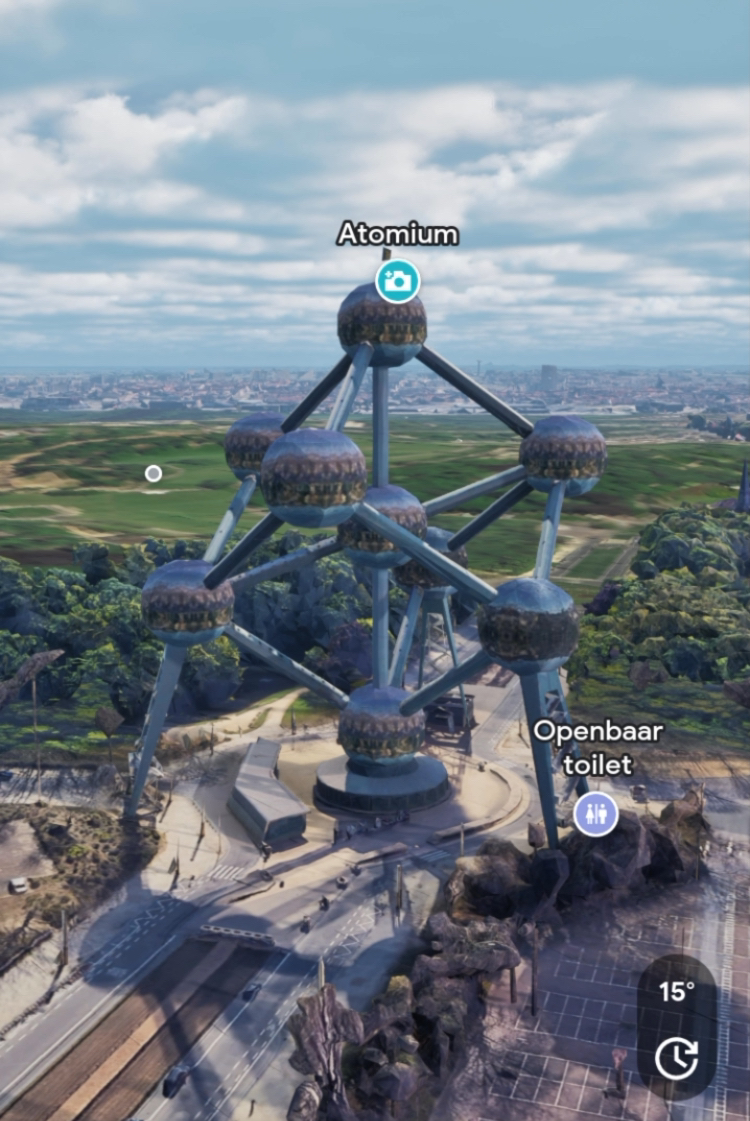
\includegraphics[width=0.5\textwidth]{IMG_1}
\caption[Immersive view Atomium Brussels]{Immersive view Atomium Brussels}
\end{figure}
\subsection{Mapbox}
\label{sec:mapbox}
Mapbox\footnote{\url{https://www.mapbox.com}} biedt een platform voor het maken en integreren van aangepaste kaarten en locatiegebaseerde services. De kaartweergave van Mapbox biedt verschillende kaartstijlen en aanpasbare kaartlagen, waardoor gebruikers een breed scala aan visuele informatie kunnen verkennen. Dit platform is ontworpen voor applicaties van derden, zo kunnen de navigatiediensten geïntegreerd worden in hun applicaties voor routebegeleiding en route-algoritmen. Mapbox heeft als groot voordeel de aanpasbaarheid per gebruiksgeval, zo kan het gemakkelijk aangepast worden naar specifieke behoeften en gebruikerservaringen. Het platform biedt AR/VR toepassingen aan, dit versterkt de leer mogelijkheden voor mensen met mentale beperking. Het grootste nadeel in deze applicatie is de afhankelijkheid van een ontwikkelaar. Ook de complexiteit die uit de applicatie komt kan mogelijke vaardigheden vereisen.
\subsection{Sygic}
\label{sec:sygic}
Sygic\footnote{\url{https://www.sygic.com/nl}} is een navigatie-app die gebruikers helpt bij het plannen van routes, navigeren op de weg en het vermijden van verkeersopstoppingen. De standaardprocedure voor het platform is je geeft je bestemming in en het programma berekent de beste route op basis van actuele verkeersinformatie. Tijdens het verplaatsen ontvangt de gebruikers stapsgewijze instructies aan de hand van spraaknavigatie, meldingen voor afslagen, rotondes en andere manoeuvres. Eens je jouw route hebt ingeladen kan je de verplaatsing offline verder zetten zonder actuele internetverbinding. Sommige geavanceerde functie van Sygic, zoals bepaalde voorkeuren instellen of het vinden van een specifiek punt. Het grootste probleem met Sygic is dat de software gebouwd is voor auto navigatie.
\subsection{De Lijn}
\label{sec:delijn}
De Lijn\footnote{\url{https://www.delijn.be/nl/routeplanner/}} staat in voor alles rond het bus en tram netwerk in Vlaanderen. Hun applicatie werkt als volgt je geeft je vertrek- en aankomstpunt in. De applicatie geeft dan een lijst terug met mogelijke bussen of trams om efficiënt op jouw bestemming te geraken. Bij het ingeven van je vertrek- en aankomstpunt geeft het ingebouwde systeem ook meteen de dichtstbijzijnde halte weer en hoe ver het wandelen is van deze halte tot je bestemming. Het systeem biedt ook real-time gegevens aan over de bussen en trams. De complexiteit van de applicatie kan een cruciale rol spelen in het verplaatsen van zichzelf en de internetverbinding die vereist is.
\subsection{NMBS}
\label{sec:nmbs}
Nationale Maatschappij der Belgische Spoorwegen (NMBS)\footnote{\url{https://www.belgiantrain.be/nl}} is de nationale treindienst van België. De grootste blokkade hier begint al bij het kennen van de vertrek en aankomsthalte. Deze applicatie biedt wel enkele voordelen zoals real-time informatie van de treintijden en het ticket systeem is in staat tickets online te bewaren. Specifieke problemen die zich hier kunnen voordoen is de complexiteit van de interface van de applicatie en een internetverbinding is vereist voor het gebruik van dit platform. In het algemeen loopt deze applicatie zeer analoog met die van De Lijn.
\section{Requirements}
\label{sec:requirements}
Bekijken welke tools voldoen aan de beste requirements 1-2 tools

Vragen aan co-promotor
\section{Het bepalen van de geschikte navigatiemethode}
\label{sec:het bepalen van de geschikte navigatiemethode}
\section{Technologieën}
\label{sec:technologieën}
\subsection{Javascript}
\label{sec:javascript}
JavaScript is een scripttaal waarmee je statische webapplicaties kunt verbeteren met
dynamische, gepersonaliseerde en interactieve inhoud. Dit verbetert de ervaring van bezoekers op uw site en
maakt het waarschijnlijker dat ze opnieuw langskomen. U hebt vast de flikkerende uitklapmenu's, bewegende
tekst en veranderende inhoud die nu wijdverspreid zijn op websites. Ze worden mogelijk gemaakt door JavaScript. JavaScript wordt ondersteund door alle grote browsers en is de taal bij uitstek op het web. Het kan zelfs worden gebruikt buiten webapplicaties, bijvoorbeeld om administratieve taken te automatiseren \autocite{Wilton2004}.
\subsection{React}
\label{sec:react}
React is een bibliotheek waarmee ontwikkelaars gebruikersinterfaces (UI's) kunnen bouwen als een boom van kleine stukjes die componenten worden genoemd. Een component is een mix van HTML en JavaScript die alle logica bevat die nodig is om een klein deel van een grotere UI weer te geven. Elk van deze componenten kan worden opgebouwd tot opeenvolgende complexe onderdelen van een app \autocite{Baer2018}.
\subsection{React Native}
\label{sec:react native}
React Native is een populair open-source framework, dat is ontwikkeld door Facebook. Ontwikkelaars kunnen hiermee mobiele applicaties bouwen aan de hand van JavaScript. React Native applicaties gebruiken de kracht van React, een JavaScript bibliotheek, voor het bouwen van gebruikersinterfaces met mobiele componenten. Door deze componenten kunnen ontwikkelaars efficiënt applicaties maken die werken voor zowel iOS als Android apparaten \autocite{Vinnik2021}.
%%=============================================================================
%% Methodologie
%%=============================================================================

\chapter{\IfLanguageName{dutch}{Methodologie}{Methodology}}%
\label{ch:methodologie}

%% TODO: In dit hoofstuk geef je een korte toelichting over hoe je te werk bent
%% gegaan. Verdeel je onderzoek in grote fasen, en licht in elke fase toe wat
%% de doelstelling was, welke deliverables daar uit gekomen zijn, en welke
%% onderzoeksmethoden je daarbij toegepast hebt. Verantwoord waarom je
%% op deze manier te werk gegaan bent.
%% 
%% Voorbeelden van zulke fasen zijn: literatuurstudie, opstellen van een
%% requirements-analyse, opstellen long-list (bij vergelijkende studie),
%% selectie van geschikte tools (bij vergelijkende studie, "short-list"),
%% opzetten testopstelling/PoC, uitvoeren testen en verzamelen
%% van resultaten, analyse van resultaten, ...
%%
%% !!!!! LET OP !!!!!
%%
%% Het is uitdrukkelijk NIET de bedoeling dat je het grootste deel van de corpus
%% van je bachelorproef in dit hoofstuk verwerkt! Dit hoofdstuk is eerder een
%% kort overzicht van je plan van aanpak.
%%
%% Maak voor elke fase (behalve het literatuuronderzoek) een NIEUW HOOFDSTUK aan
%% en geef het een gepaste titel.

%%\lipsum[21-25]
De methodologie van dit onderzoek naar navigatiemethoden voor mensen met een mentale beperking is opgedeeld in drie belangrijke fasen, elk essentieel voor het bereiken van de onderzoeksdoelstellingen: een literatuurstudie, een requirementsanalyse en de uitwerking van een Proof of Concept (PoC). Dankzij de requirementsanalyse is een long list van methoden ingekort tot een short list van diegenen best in aanmerking konden komen voor de doelgroep. De vergelijkende studie van deze shortlist is besproken in de resultatenverwerking en heeft aanleiding gegeven tot enkele gerichte conclusies, waarmee de scriptie is afgerond onder de vorm van enkele aanbevelingen.

\subsection*{Mapping}
De eerste fase heeft bestaan uit een uitgebreide literatuurstudie waarin de basisbegrippen van navigatie en ondersteunende technologieën in kaart worden gebracht, evenals de concrete definitie van de impact van een mentale beperking op het gebruik hiervan.  Door bestaande navigatiemethoden en -tools te bestuderen, is hun toepasbaarheid en effectiviteit voor onze specifieke doelgroep geëvalueerd. De hoofdvraag is daarom opgesplitst in diverse deelaspecten. Kan locatiebepaling helpen om zelfstandige input van de gebruikers te omzeilen ? Kan de integratie van AR een toegevoegde waarde bieden omtrent veiligheidsgevoel en comfort ? Welke specifieke communicatiemogelijkheden voor mensen met een beperking zijn bruikbaar? Deze fase is cruciaal geweest voor het beantwoorden van de deelvraag over het huidige landschap van navigatiehulpmiddelen, meerbepaald het identificeren van eventuele lacunes in de bestaande technologieën. Het eindresultaat is een mapping die kan afgetoetst worden in functie van de gebruikersnoden en als input heeft gediend voor de requirementsanalyse.

\subsection*{Requirementsanalyse en Long List}

Na het opbouwen van een theoretisch kader, is gestart met de tweede fase, namelijk een vergelijkende studie van de geïdentificeerde navigatiemethoden. Hierbij is gebruik gemaakt van de MoSCoW-methode om prioriteit te geven aan verschillende requirements die essentieel zijn voor de doelgroep. Ze heeft rekening gehouden met een aantal functies, integraties en mogelijke werkwijzen zoals hieronder opgelijst:

\begin{enumerate}
    \item \textbf{Functies}: Een lijst van alle nodige functies in de app bv. location tracking, text-to-speech, voorleesfunctie, language models, visualisatietypes, Sclera pictogrammen
    \item \textbf{Integraties}: Een omschrijving van mogelijke AR integraties
    \item \textbf{Werkwijze en denkpatronen}: Een selectie van enkele mogelijke manieren waarmee interactie kan geïnitieerd worden inclusief AR (kleuren, geluiden, patronen, figuren, $\ldots$)
\end{enumerate}

Er is bepaald welke criteria 'Must Have', 'Should Have', 'Could Have' en 'Won't Have' zijn. Alleen de mogelijkheden die voldoen aan de 'Must Have'-criteria werden geselecteerd voor verdere evaluatie. Dit heeft ervoor gezorgd dat de gekozen methoden niet alleen technisch haalbaar zijn, maar ook maximaal aansluiten bij de behoeften van mensen met een mentale beperking. Zij hebben de basis gevormd van de proof of concept.

\subsection*{Proof of Concept en Short List}

In de derde en laatste fase is een proof of concept ontwikkeld door twee geselecteerde navigatiemethoden te evalueren voor de opbouw van een testapplicatie. De POC is uitgewerkt voor een smartphone voor een aantal specifieke routes. Deze applicatie is ontwikkeld in React Native om de functionaliteit en gebruikerservaring te evalueren in functie van de doelgroep. Het gedeelte waarin data wordt verzameld over bruikbaarheid, toegankelijkheid en effectiviteit door middel van directe observaties en gebruikersfeedback, en waar een data-analyse wordt uitgevoerd van de tijd nodig voor verplaatsing van punt A naar punt B zonder en met gebruik van de applicatie, is vervangen door een gedetailleerde evaluatie van de navigatiemethoden. Deze evaluatie omvat de identificatie van de meest geschikte navigatiemethoden op basis van de criteria vastgesteld in de tweede fase, en de aanbevelingen van specifieke technologieën en benaderingen die het beste voldoen aan de behoeften van de doelgroep. Dit houdt in dat de nadruk verschuift van het simpelweg meten van reistijd en gebruikerservaring naar een bredere analyse en aanbeveling van navigatiemethoden en technologieën die het meest effectief zijn voor mensen met een mentale beperking.

\subsection*{Resultatenverwerking, evaluatie en aanbevelingen}

De uitkomst van deze vergelijking is gebruikt om de meest geschikte navigatiemethode(s) te identificeren die best voldoen aan de behoeften van onze doelgroep, gebaseerd op de criteria vastgesteld in fase 2. Daaruit zijn essentiële conclusies gevolgd nodig voor het aanbevelen van specifieke navigatietechnologieën en -benaderingen die kunnen worden geïmplementeerd in mobiliteitstools voor mensen met een mentale beperking, waarbij gestreefd wordt naar het verbeteren van hun zelfstandigheid en kwaliteit van leven.


%%=============================================================================
%% Proof of Concept
%%=============================================================================

\chapter{\IfLanguageName{dutch}{Proof of Concept}{Proof of Concept}}%
\label{ch:proof-of-concept}

In dit deel van het onderzoek presenteert een proof of concept gericht op de beoordeling van de gekozen navigatiemethoden, die gebruikt kunnen worden voor mensen met een mentale beperking. Het doel van de proof of concept is de efficiëntie, bruikbaarheid en gebruiksvriendelijkheid van deze methoden te onderzoeken aan de hand van een applicatie. De ontwikkeling van deze applicatie en hieruit gehaalde resultaten worden besproken. Als laatste zal er een discussie worden gevoerd, welke navigatietool de meest geschikte is voor de doelgroep.

\section{Ontwikkeling van de applicatie}
\label{sec:ontwikkeling van de applicatie}
In dit onderdeel wordt de opbouw van de applicatie besproken. Hieruit zal duidelijk worden hoe de applicatie opgebouwd is. De code is niet relevant voor het verdere verloop van het onderzoek. Als eerste worden de belangrijkste onderdelen besproken. Een nieuw React Native project wordt aangemaakt aan de hand van Node.js en een terminal. Na het opzetten van dit project, moet er een Mapbox account gecreëerd worden voor een publieke token zodat er gebruik gemaakt kan worden van hun diverse mappen. \newline

In de applicatie is één simpel scherm. Op Figuur \ref{fig:Scherm met een knop om de route op te vragen} is te zien dat er een Mapbox map ingeladen wordt en een invoerveld met een knop. Het proces wordt in gang gezet wanneer op de knop gedrukt wordt en een correct adres is ingegeven. Wanneer een foutief adres wordt ingegeven zal er een foutmelding komen en wordt het proces onderbroken. Bij Figuur \ref{fig:Scherm met knop waar route die opgevraagd is} 

\begin{lstlisting}[caption={Code-voorbeeld van het navigatiescherm}, label=code-voorbeeld navigatiescherm, captionpos=b]
    Mapbox.setAccessToken('MAPBOX_PUBLIC_TOKEN');
    
    const App = () => {
        const [location, setLocation] = useState('');
        const [destination, setDestination] = useState('');
        const [route, setRoute] = useState(null);
        const [errorMsg, setErrorMsg] = useState(null);
        const [isLoading, setIsLoading] = useState(false);
        
        useEffect(() => {
            (async () => {
                let { status } = await Location.requestForegroundPermissionsAsync();
                if (status !== 'granted') {
                    setErrorMsg('Permission to access location was denied');
                    return;
                }
                
                let currentLocation;
                if (Platform.OS === 'OS' && !__DEV__) {
                    currentLocation = await Location.getCurrentPositionAsync({});
                    console.log('Current location:', currentLocation);
                } else {
                    currentLocation = {
                        coords: {
                            longitude: 4.038139399999999,
                            latitude: 50.9318886,
                        },
                    };
                }
                
                if (!currentLocation) {
                    setErrorMsg('Failed to obtain location');
                    return;
                }
                setLocation(currentLocation);
            })();
        }, []);
        
        const getRoute = async () => {
            setIsLoading(true);
            const userLocation = `${location.coords.longitude},${location.coords.latitude}`;
            console.log('User location:', userLocation);
            
            const YOUR_GOOGLE_API_KEY = 'GOOGLE_API_KEY';
            
            const startLong = location.coords.longitude;
            const startLat = location.coords.latitude;
            
            try {
                const destinationCoords = await getCoordinatesFromPlace(destination, YOUR_GOOGLE_API_KEY);
                const endLong = destinationCoords.split(',')[1];
                const endLat = destinationCoords.split(',')[0];
                console.log(endLong, endLat)
                console.log('Destination coordinates:', destinationCoords);
                if(!destinationCoords) {
                    throw new Error('Failed to fetch destination coordinates');
                }
                
                const mapboxUrl = `https://api.mapbox.com/directions/v5/mapbox/walking/${startLong},${startLat};${endLong},${endLat}?alternatives=true&annotations=distance&continue_straight=true&geometries=geojson&overview=full&steps=false&access_token=MAPBOX_PUBLIC_TOKEN`
                console.log('Mapbox Directions API URL:', mapboxUrl);
                const response = await fetch(mapboxUrl);
                const data = await response.json();
                                
                if (data.routes && data.routes.length > 0) {
                    const routeCoordinates = data.routes[0].geometry.coordinates.map(coord => ({ longitude: coord[0], latitude: coord[1] }));
                    // console.log('Route coordinates:', routeCoordinates);
                    setRoute(routeCoordinates);
                } else if (data.coords == 'NoRoute'){
                    throw new Error('No route found');
                } else {
                    throw new Error('Failed to fetch route');
                }
            } catch (error) {
                console.error(error);
                setErrorMsg('Failed to fetch route');
            } finally {
                setIsLoading(false);
            }
        };
        
        const getCoordinatesFromPlace = async (place, apiKey) => {
            const apiUrl = `https://maps.googleapis.com/maps/api/geocode/json?address=${encodeURIComponent(place)}&key=${apiKey}`;
            
            try {
                const response = await fetch(apiUrl);
                
                console.log('Geocoding API response status:', response.status);
                
                if (!response.ok) {
                    throw new Error(`Geocoding API request failed with status ${response.status}`);
                }
                
                const data = await response.json();
                                
                if (data.status === 'OK' && data.results.length > 0) {
                    const result = data.results.find(result => result && result.geometry && result.geometry.location);
                    if (result) {
                        const { lat, lng } = result.geometry.location;
                        console.log('Geocoding result:', lat, lng);
                        return `${lat},${lng}`;
                    } else {
                        throw new Error('No valid location found in the geocoding results');
                    }
                } else {
                    throw new Error(`Geocoding failed: ${data.status || 'Unknown error'}`);
                }
            } catch (error) {
                console.error('Error in getCoordinatesFromPlace:', error);
                throw error;
            }
        };
        
        const renderRouteLine = () => {
            if (!route) {
                return null; 
            }
            
            const routeCoordinates = route.map(coord => [coord.longitude, coord.latitude]);
            // console.log("Route coordinates:", route);
            return (
            <Mapbox.ShapeSource id="routeSource" shape={{
                    type: 'Feature',
                    geometry: {
                        type: 'LineString',
                        coordinates: routeCoordinates,
                    },
            }}>
            <Mapbox.LineLayer id="routeFill" style={{ lineColor: 'blue', lineWidth: 3 }} />
            </Mapbox.ShapeSource>
            );
        };
        
        if (!location || !location.coords) {
            return (
            <View style={styles.container}>
            <ActivityIndicator size="large" />
            <Text>{errorMsg || 'Waiting for location...'}</Text>
            </View>
            );
        }
        
        return (
        <View style={styles.container}>
        <Mapbox.MapView style={styles.map}>
        <Mapbox.Camera
        zoomLevel={13}
        centerCoordinate={[location.coords.longitude, location.coords.latitude]}
        />
        <Mapbox.UserLocation />
        {route && renderRouteLine()}
        </Mapbox.MapView>
        
        {/* Destination Input Field */}
        <View style={styles.inputContainer}>
        <TextInput
        style={styles.input}
        placeholder="Enter destination address"
        value={destination}
        onChangeText={setDestination}
        />
        <Button title="Get Route" onPress={getRoute} disabled={isLoading} />
        </View>
        
        {isLoading && (
            <View style={styles.loading}>
            <ActivityIndicator size="large" />
            </View>
            )}
        </View>
        );
    };
    
    export default App;
    
    const styles = StyleSheet.create({
        container: {
            ...StyleSheet.absoluteFillObject,
            justifyContent: 'flex-end',
            alignItems: 'center',
        },
        map: {
            ...StyleSheet.absoluteFillObject,
        },
        inputContainer: {
            width: '100%',
            marginBottom: 20,
        },
        input: {
            width: '90%',
            paddingHorizontal: 10,
            borderWidth: 1,
            borderColor: '#ccc',
            borderRadius: 5,
            height: 40,
            backgroundColor: '#fff',
            marginBottom: 10,
        },
        loading: {
            position: 'absolute',
            top: '50%',
            left: '50%',
            zIndex: 1,
            transform: [{ translateX: -25 }, { translateY: -25 }],
        },
    });
\end{lstlisting}

\begin{figure}[htbp]
    \centering
    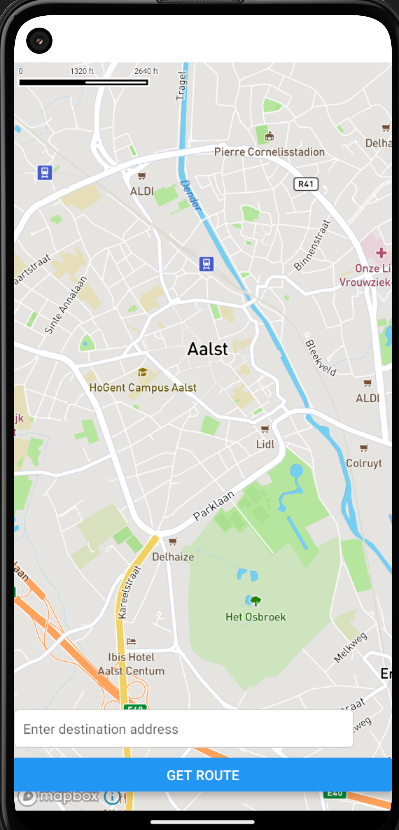
\includegraphics[width=0.5\textwidth]{image.png}
    \caption{Scherm met een knop om de route op te vragen}
    \label{fig:Scherm met een knop om de route op te vragen}
\end{figure}

\begin{figure}[htbp]
    \centering
    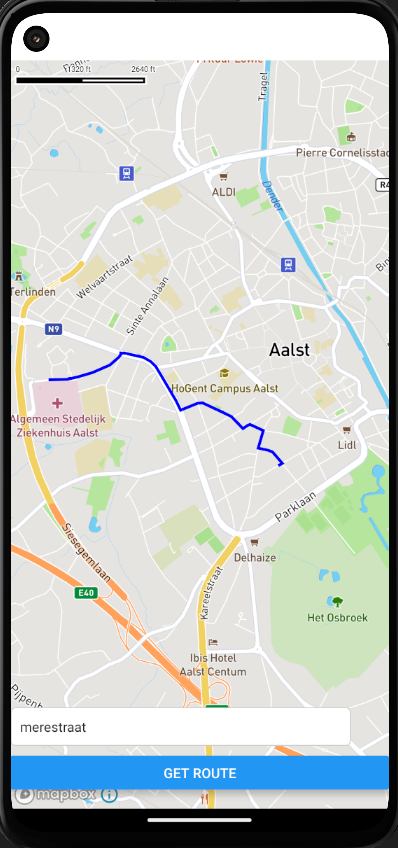
\includegraphics[width=0.5\textwidth]{image-1.png}
    \caption{Scherm met knop waar de route die opgevraagd is}
    \label{fig:Scherm met knop waar route die opgevraagd is}
\end{figure}

\subsection{Installatie en opstarten van de applicatie}
\label{sec:installatie en opstarten van de applicatie}

Zorg ervoor dat Node.js geïnstalleerd is op je systeem en in je \texttt{\$PATH} variabelen staat.
een Mapbox publieke token is nodig om de kaarten te kunnen gebruiken.

\begin{enumerate}
    \item Clone de repository.
    \item Voer `npm install` uit in de hoofdmap van de repository.
    \item In \texttt{App.js}, vervang \texttt{Mapbox.setAccessToken('YOUR\_MAPBOX\_PUBLIC\_KEY');} door je eigen Mapbox publieke token.
    \item Bij \textbf{MapboxUrl} in \texttt{App.js}, vervang \texttt{access\_token=YOUR\_MAPBOX\_PUBLIC\_KEY} aan het einde van de URL met je eigen Mapbox publieke token.
    \item Je hebt ook een \textbf{Google API key} \texttt{YOUR\_GOOGLE\_API\_KEY} nodig voor het maken van de route. Deze kan je verkrijgen op de Google Cloud Platform\footnote{\url{https://cloud.google.com/?hl=nl}}.
    \item Voer `npx expo start` uit om de applicatie te starten. Je kan de optie \texttt{--android} of \texttt{--ios} toevoegen om de applicatie te starten in een specifieke emulator.
    \item Selecteer een emulator of scan de QR code met de Expo app op je telefoon.
\end{enumerate}

\section{Praktijkonderzoek}
\label{sec:praktijkonderzoek}

%mapbox getest

%google maps getest functies

\section{Discussie}
\label{sec:discussie}

inleiding

\subsection{Resultaten}
\label{sec:resultaten}

vergelijkingen en bemerkingen van de applicaties

\subsection{Alternatief}
\label{sec:alternatief}

Voor mapbox wat kan je doen

\subsection{Reflectie}
\label{sec:reflectie}

Eigen reflectie voor gebruik

% Voeg hier je eigen hoofdstukken toe die de ``corpus'' van je bachelorproef
% vormen. De structuur en titels hangen af van je eigen onderzoek. Je kan bv.
% elke fase in je onderzoek in een apart hoofdstuk bespreken.

%\input{...}
%\input{...}
%...

%%=============================================================================
%% Conclusie
%%=============================================================================

\chapter{Conclusie}%
\label{ch:conclusie}

% TODO: Trek een duidelijke conclusie, in de vorm van een antwoord op de
% onderzoeksvra(a)g(en). Wat was jouw bijdrage aan het onderzoeksdomein en
% hoe biedt dit meerwaarde aan het vakgebied/doelgroep? 
% Reflecteer kritisch over het resultaat. In Engelse teksten wordt deze sectie
% ``Discussion'' genoemd. Had je deze uitkomst verwacht? Zijn er zaken die nog
% niet duidelijk zijn?
% Heeft het onderzoek geleid tot nieuwe vragen die uitnodigen tot verder 
%onderzoek?

\lipsum[76-80]



%---------- Bijlagen -----------------------------------------------------------

\appendix

\chapter{Onderzoeksvoorstel}

Het onderwerp van deze bachelorproef is gebaseerd op een onderzoeksvoorstel dat vooraf werd beoordeeld door de promotor. Dat voorstel is opgenomen in deze bijlage.

%% TODO: 
%\section*{Samenvatting}

% Kopieer en plak hier de samenvatting (abstract) van je onderzoeksvoorstel.

% Verwijzing naar het bestand met de inhoud van het onderzoeksvoorstel
%---------- Inleiding ---------------------------------------------------------

\section{Introductie}%
\label{sec:introductie}

    personen met een mentale beperking ondervinden bij het gebruik van bestaande mobiliteits\-tools problemen, omdat deze uitgaan van een basisniveau lees- en schrijfvaardigheid waarover zij dikwijls niet beschikken. 
    Bovendien is in sommige gevallen ook hun tijds- en ruimtebesef gelimiteerd. 
    Het globale objectief van het onderzoek is een tool te ontwikkelen om deze doelgroep via Augmented Reality (AR) ondersteuning te bieden om bestaande mobiliteitstools op een efficiënte en veilige manier te gebruiken.
    De Proof-of-Concept (POC) wordt zo eenvoudig mogelijk ontwikkeld, zodat ze gestructureerd hun weg kunnen vinden met behulp van het openbaar vervoer. 
    Door bestaande tools te screenen, al dan niet gericht op onze doelgroep, en deze af te toetsen door bevraging van verschillende stakeholders, wordt een meer optimale tool in kaart gebracht. 
    Kort gezegd: hoe geraakt iemand die niet kan (klok)lezen zonder enige begeleiding van punt A naar punt B met visuele en/of auditieve signalen aan de hand van AR binnen het juiste tijdsbestek? We zijn ervan overtuigd dat deze mobiliteitstool een grote impact en meerwaarde zal hebben voor deze doelgroep door hun grenzen te verleggen en zelfstandigheid te vergroten. De hoofdvraag kan hiertoe in enkele deelvragen onderverdeeld worden;
    
    \begin{enumerate}
        \item Welke problemen ervaren personen met een mentale beperking bij het gebruik van bestaande mobiliteitstools?
        \item Hoe kan Augmented Reality (AR) ge-\\integreerd worden in bestaande mobiliteits\-tools?
        \item Hoe kunnen AR en locatiebepaling worden ingezet om personen met een mentale beperking te ondersteunen bij het navigeren met het openbaar vervoer?
        \item Op welke manieren kan de mobiliteitstool worden aangepast aan de specifieke behoeften en voorkeuren van de doelgroep?
        \item Hoe kan een praktijkexperiment worden opgezet om de efficiëntie en gebruiksvriendelijkheid van de ontwikkelde mobiliteitstool te evalueren bij de doelgroep?
        \item Welke visuele en/of auditieve signalen zijn het \\meest efficiënt?
    \end{enumerate}

%---------- Stand van zaken ---------------------------------------------------

\section{State-of-the-art}%
\label{sec:state-of-the-art}
  
  De literatuurstudie zal zich richten op het verkennen van de mobiliteitsbehoeften van de doelgroep en het bespreken van bestaande tools en technologieën die hen kunnen ondersteunen bij het navigeren en reizen.
  Mensen met een beperking worden vaak geconfronteerd met uitdagingen bij het plannen en uitvoeren van verplaatsingen. Afhankelijk van hun type beperking kunnen deze noden bovendien sterk variëren. Bij autismespectrumstoornis (ASS) werden diverse aspecten omtrent tijdsbesef samengevat door Prof. Degrieck \autocite{Degrieck2014}.
  Een grote gemeenschappelijke deler bij deze doelgroep is de nood aan eenduidige structuur, vaak visueel ondersteund en de afwezigheid van onnodige prikkels. De website van Participate\footnote{\url{https://nl.participate-autisme.be}} bundelt hieromtrent heel wat ervaringsgerichte informatie via hun FAQ en enkele blogs. Zeker in de context van ASS is een advertentie-luwe omgeving met enkel essentiële informatie een absolute noodzaak \autocite{Roeyers2014}. 
  De mogelijkheid om te kiezen voor een klassiek klokbeeld in plaats van het digitale beeld of een keuze voor bepaalde lettertypes kan voor mensen met een laag IQ die slechts bepaalde letter- en cijfercombinaties kunnen memoriseren het verschil maken \autocite{Uyttersprot2021,Tytgat2014,DeGraaf2001}. Welke technologieën dragen het beste bij tot begrijpbaarheid en kunnen zo hun mobiliteit en zelfstandigheid verbeteren?
  Een aantal belangrijke aandachtspunten en best practices voor mensen met een beperking zullen vanuit deze invalshoeken worden onderzocht, zoals de noodzaak van locatiegebaseerde informatie, de mogelijkheid van het gebruik van pictogrammen voor het beschrijven van locaties, en de integratie van spraakherkenning voor gebruikers die niet kunnen lezen of schrijven.Daarnaast zullen verschillende soorten mobiliteitsapps worden besproken, waaronder applicaties van openbare vervoersmaatschappijen zoals NMBS\footnote{\url{https://www.belgiantrain.be/nl}} en De Lijn\footnote{\url{https://www.delijn.be/nl/}}, standaard routeplanners en andere specifieke mobiliteitsapps zoals Dott\footnote{\url{https://ridedott.com/nl/}} en Villo\footnote{\url{https://www.villo.be/nl/home}} voor fietsen en steps. Het doel is om te analyseren hoe deze apps momenteel functioneren en welke verbeteringen nodig zijn om ze toegankelijker te maken voor mensen met een beperking.
  Deze applicaties en websites zijn gebaseerd op het principe dat de gebruiker zelfstandig een adres en tijdstip zelf kan ingeven en maken niet altijd gebruik van locatiebepaling, wat voor de doelgroep een duidelijke hinderpaal is.
  Daarnaast zullen diverse Augmented Reality (AR) methodes binnen de huidige state of the art vergeleken worden voor het verbeteren van de gebruikerservaring.
  Mapbox AR\footnote{\url{https://www.mapbox.com/augmented-reality}} maakt gebruik van points of interest terwijl Google Maps AR \footnote{\url{https://arvr.google.com}} inzet op multidimensionele visualisatie om de gebruiker comfortabel aan te sturen tijdens het navigeren.
  Met behulp van de camera van het mobiele apparaat worden real-time beelden van de omgeving vastgelegd, waarbij digitale routeaanwijzingen over de werkelijke beelden worden geprojecteerd.
  Dit zorgt voor een intuïtieve en praktische navigatie-ervaring, vooral in stedelijke gebieden waar traditionele kaarten mogelijk minder effectief zijn.
  Mapbox AR onderscheidt zich door zijn typische karakteristiek van geavanceerde aanpasbaarheid en integratiemogelijkheden.
  Deze tool biedt ontwikkelaars een krachtig platform waarmee ze op maat gemaakte augmented reality-toepassingen kunnen creëren, variërend van navigatie tot locatiegebaseerde informatie.
  Hierdoor hebben ontwikkelaars de flexibiliteit om kaartgegevens aan te passen, aangepaste overlays toe te voegen en de gebruikerservaring te optimaliseren voor specifieke doeleinden.
  Beide tools vertegenwoordigen technologieën binnen het domein van augmented reality en kaartnavigatie. Ze tonen de evolutie aan van traditionele kaartapplicaties naar meer dynamische, op AR gebaseerde oplossingen.
  Ook Koombea\footnote{\url{https://www.koombea.com}} verhoogt de gebruikerservaring en met AR City\footnote{\url{https://arcitygame.nl}} komt de locatie effectief tot leven dankzij bijkomende informatie.
  Sygic\footnote{\url{https://www.sygic.com}} werd specifiek ontwikkeld voor auto GPS-systemen om de bestuurderservaring te optimaliseren, maar kan een toegevoegde waarde hebben wanneer de gebruiker tijdens een busrit het traject mee wil opvolgen.
  De implementatie van locatiegevoelige informatie in combinatie met de AR visualisatie neemt diverse barrières weg voor de doelgroep.
  Zij hoeven immers niet het adres te kennen van hun startpunt. Het eindpunt kunnen ze bv. omschrijven via een pictogram zoals deze gebruikt worden in Sclera\footnote{\url{https://www.sclera.be/nl/picto/overview}}.
  Deze pictogrammen worden standaard aangeleerd bij onze doelgroep ter bevordering van hun communicatie en visualisatie van hun dagplanning.
  Naast het openbaar vervoer kunnen andere systemen zoals Dott en Villo worden overwogen omdat dergelijke fietsen en steps verspreid staan in diverse steden.
  Ze bieden een bijkomende optie voor het verplaatsen van punt A naar punt B op een efficiënte manier.
  Op hardwaregebied ontwikkelde Google in 2014 een smart device genaamd Google Glasses.
  Deze brillen hadden als doel om AR een extra boost te geven aan de hand van een concreet concept.
  Het product kreeg een tweede versie in 2017, als ondernemingseditie, maar had geen succes en eerder dit jaar in maart 2023 kondigde Google aan dat ze het project stopzetten \autocite{Gvora2023}.
  Tot slot geldt dat de doelgroep die niet in staat is te lezen of schrijven, wel gebruik kan maken van text-to-speech functionaliteit om de gewenste locatie te omschrijven.
  De tool moet met andere woorden ook deze stemherkenning als ondersteuning bieden.
  Dankzij artificiële intelligentie (AI) wordt dan de relatief beste route berekent en tevens de beste manier om daar eenvoudig te geraken \autocite{Soni2023a}.
  Het gebruik van datastructuren zal toelaten deze locatie informatie te linken aan het routepatroon \autocite{Ruta2010}.
  Bovendien kunnen deze patronen potentiële knelpunten identificeren, hulp bieden bij het optimaliseren van routes als er verkeerswerken of files zijn.
  De noodzaak van dit systeem zijn realtime gegevens waarbij samenwerking met belanghebbende belangrijk is \autocite{Ciravegna2018}.
  Het opzetten van een meta model kan begeleiders van mensen met een matige mentale beperking helpen met het navigeren naar een juiste plaats.
  Door gegevensverzameling kan er aan de hand van algoritmes voorspellingen gemaakt worden wat voor deze persoon de favoriete manier van verplaatsen is of favoriete route is om te volgen naar het werk \autocite{Stepanov2003}.
  Als laatste kan er gebruik gemaakt worden van Internet of Things (IoT) tools voor het slim communiceren tussen verschillende apparatuur wat kan leiden tot nog betere prestaties in verplaatsing en routeberekening \autocite{Fatnassi2015}.

% Voor literatuurverwijzingen zijn er twee belangrijke commando's:
% \autocite{KEY} => (Auteur, jaartal) Gebruik dit als de naam van de auteur
%   geen onderdeel is van de zin.
% \textcite{KEY} => Auteur (jaartal)  Gebruik dit als de auteursnaam wel een
%   functie heeft in de zin (bv. ``Uit onderzoek door Doll & Hill (1954) bleek
%   ...'')

%---------- Methodologie ------------------------------------------------------
\section{Methodologie}%
\label{sec:methodologie}

De methodologie van het onderzoek bestaat uit een aantal belangrijke deelstappen waaronder literatuurstudie, een requirementsanalyse door middel van bevraging van de noden bij de stakeholders, definitie van de software inclusief Augmented Reality (AR) opties, mogelijke hardwarecomponenten voor implementatie, uitwerking van de Proof-of-Concept (POC), een praktijkexperiment in meerdere fasen, het formuleren van de conclusies en de scriptie. De hoofdvraag omvat diverse deelaspecten zoals ``kan locatiebepaling helpen om zelfstandige input van de gebruikers te omzeilen''. Anderzijds zal ook het deelaspect van de specifieke communicatiemogelijkheden voor mensen met een beperking worden geëvalueerd. Tot slot brengt de integratie van AR een toegevoegde waarde omtrent veiligheidsgevoel en comfort, wat moet blijken uit de feedback van de praktijktesten. Na de nodige research online en in bestaande applicaties van huidige aanbieders, is een bevraging van diverse stakeholders gepland. Aan de hand van interviews met Fiola\footnote{\url{https://fiolavzw.be}} (begeleiding mensen met mentale beperking), Tanderuis\footnote{\url{https://www.tanderuis.be}} (gespecialiseerd in autismespectrumstoornis), begeleidingsorganisaties en vakexperten die mensen met een matige mentale beperking begeleiden, worden inzichten verworven over de huidige mogelijkheden en de specifieke noden. Welke zijn de basisvoorwaarden voor een toegankelijke applicatie en welke aangepaste communicatiemiddelen kunnen praktisch ingezet worden. Deze bevraging zal het lastenboek definiëren voor onze POC en mogelijkheden voor samenwerking verduidelijken.
Functionaliteiten van elk deze tools zullen gescreend worden om te bepalen of zij in aanmerking komen voor integratie in de POC.
Voor het evalueren van de mobiliteitstool zullen praktijktesten worden uitgevoerd, waarbij de tijd die nodig is voor de verplaatsing van punt A naar punt B centraal staat. 
Deze testen zullen gebaseerd zijn op tijdmetingen, waarbij zowel een nulmeting zonder gebruik van de applicatie als met de mobiliteitstool zal worden uitgevoerd. We zullen bij de nulmeting ook hun route traceren.
Het doel van deze tests is om inzicht te krijgen in de effectiviteit van de mobiliteitstool in het verminderen van de benodigde tijd voor verplaatsingen en om eventuele verbeteringen te identificeren. 
De resultaten zullen worden verwerkt door het berekenen van gemiddelden, het analyseren van de spreiding van de data en het identificeren van eventuele verbeteringen ten opzichte van de nulmeting. Deze gegevens zullen cruciaal zijn voor het beoordelen van de effectiviteit van de mobiliteitstool en het informeren van verdere ontwikkelingen en aanpassingen. De POC zal worden uitgewerkt op een smartphone voor een aantal specifieke routes waarin minstens 1 openbaar vervoersmiddel (trein, bus, tram, ...) is geïntegreerd. Uiteindelijk zal een compilatie gemaakt worden van de beste opties en combinaties om verder uit te werken in de POC; 

\begin{enumerate}
    \item \textbf{Functies}: Een lijst van alle nodige functies in de app (location tracking, text-to-speech, voorleesfunctie, language models, visualisatietypes, Sclera pictogrammen)
    \item \textbf{Integraties}: Een omschrijving van mogelijke AR integraties (Google Maps, Mapbox, Koombea, AR City, Sygic)
    \item \textbf{Werkwijze en denkpatronen}: Een selectie van enkele mogelijke manieren waarmee interactie kan geïnitieerd worden inclusief AR (kleuren, geluiden, patronen, figuren, ...)
\end{enumerate}


%---------- Verwachte resultaten ----------------------------------------------
\section{Verwacht resultaat, conclusie}%
\label{sec:verwachte_resultaten}

Uit de screening van bestaande tools zullen nuttige functies worden gebruikt als bouwstenen voor de Proof-of-Concept (POC) van dit onderzoek. 
Dankzij de inzichten verworven in de bevraging van de noden en gesprekken met diverse stakeholders zal deze POC zo functioneel mogelijk zijn voor de specifieke doelgroep. 
Tot slot zal dankzij een experimentele fase nagegaan worden hoe efficiënt de concrete uitwerking is en welke positieve impact Augmented Reality (AR) implementatie kan hebben.
In essentie kan worden gesteld dat er al enkele bruikbare tools ontwikkeld zijn, maar deze niet (volledig) aan de noden voldoen voor mensen met een matige mentale beperking. Deze hulpmiddelen vereisen nog steeds een redelijke kennis in het gebruik. Daarom wordt, na bevragingen, een POC opgesteld aan de hand van verworven inzichten. De bekomen resultaten van de literatuurstudie, in combinatie met de bevragingen en gebouwde POC, zullen een duidelijk beeld schetsen voor de samenwerking met een hardwarebedrijf of AR bedrijf. 
Als resultaat hierop wordt meteen ook nagedacht over extra functies en integraties die dan samengevat worden als opsomming met latere innovaties.



%%---------- Andere bijlagen --------------------------------------------------
% TODO: Voeg hier eventuele andere bijlagen toe. Bv. als je deze BP voor de
% tweede keer indient, een overzicht van de verbeteringen t.o.v. het origineel.
%\input{...}

%%---------- Backmatter, referentielijst ---------------------------------------

\backmatter{}

\setlength\bibitemsep{2pt} %% Add Some space between the bibliograpy entries
\printbibliography[heading=bibintoc]

\end{document}
